
\subsection{Authentication Enforcer} 
\begin{flushleft}
The Authentication Enforcer pattern handles the authentication logic across all of the actions within the Web tier. It assumes responsibility for authentication and verification of user identity and delegates direct interaction with the security provider to a helper class. This applies not only to password-based authentication, but also to client certificate-based authentication and other authentication schemes that provide a user's identity, such as Kerberos.
This pattern will help us improve security of the system while keeping the scalability and performance well maintained since the Authentication Enforcer pattern provides a consistent and structured way to handle authentication and verification of requests across actions within Web-tier components and also supports MVC architecture without duplicating the code.
\end{flushleft}

\subsection{Dependency Injection}
\begin{flushleft}
Dependency injection implements inversion of control for software libraries.\\
The design pattern allows a client to remove all
knowledge of a concrete implementation that it needs to use. This helps isolate the client
from the impact of design changes and defects. It promotes re-usability, testability and
maintainability.
The benefits of using Dependency Injection in our system, is that it will ensure loose coupling of code between the different modules that need to be implemented. Decoupling of code will ensure that the code in the system are cleaner, easier to modify when required and easier to adapt and implement for reuse.
\end{flushleft}

\subsection{Flyweight Design Pattern}
\begin{flushleft}
A flyweight is an object that minimizes memory use by sharing as much data as possible with other similar objects; it is a way to use objects in large numbers when a simple repeated representation would use an unacceptable amount of memory. This is how we will improve on performance and the scalability of the system as resources are used efficiently and effectively.
\end{flushleft}

\subsection {Mock Object}
Mock objects are simulated objects that mimic the behavior of real objects in controlled ways.
We have to create a mock object to test the behavior of some other object and see how it reacts
to certain conditions.

\subsection {Model-View-Controller (MVC)}

\begin{flushleft}

Adhering to the MVC design pattern provides us with numerous benefits:

\begin{enumerate}
	\item \textbf{Separation of design concerns:} Because of the decoupling of presentation, control, and data persistence and behavior, the application becomes more flexible; modifications to one component have minimal impact on other components.
	\item \textbf{More easily maintainable and extensible:} Good structure can reduce code complexity. As such, code duplication is minimized.
	\item \textbf{Promotes division of labour:}Developers with different skill sets are able to focus on their core skills and collaborate through clearly defined interfaces.
\end{enumerate}

	\begin{figure}[H]
		\centering\graphicspath{ {images/} }
		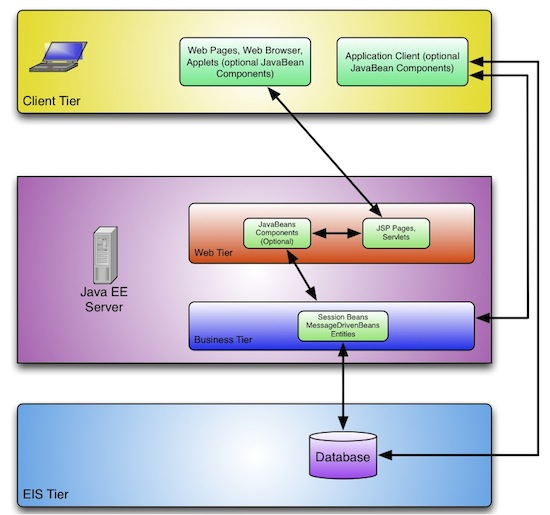
\includegraphics[width=\textwidth,height=15cm]{MVC.jpg}
	   	\caption{Java-EE system architecture}
	\end{figure}

\textbf{View (Client Tier)}\\
This tier runs on the user system and encapsulates the various components that a user system may use to access the Java EE server-side tiers. These components include dynamic web pages, Java applications and Java applets.

\textbf{Controller (Java-EE server)}

The middle tier's business functions handle client requests and process application data, storing it in a permanent data store in the data tier.

\begin{itemize}
	\item \textbf{Web Tier}
	\\The web tier consists of components that handle the interaction between clients and the business tier.
	
	\item \textbf{Business Tier}
	\\The business tier consists of components that provide the business logic for an application. Business logic is code that provides functionality to a particular business domain.
\end{itemize}

\textbf{Model (Enterprise Information Systems (EIS) Tier)}\\
The EIS tier consists of database servers, enterprise resource planning systems, and other legacy data sources. These resources typically are located on a separate machine than the Java EE server, and are accessed by components on the business tier. This will be the university's server for the mini project.

\end{flushleft}






